\subsubsection{usergoal-ugManageCrisis}

\label{RE-use-case-ugManageCrisis}


The goal is to do an action that makes the handling of a crisis or an alert progress.		  


\begin{usecase}
  \addheading{Use-Case Description}
  \addsingletwocolumnrow{Name}{ugManageCrisis}
  \addsingletwocolumnrow{Scope}{system}
  \addsingletwocolumnrow{Level}{usergoal}
  

\addrowheading{Primary actor(s)}
\addnumberedsinglerow{}{\msrcode{actCoordinator[active]}}



\addrowheading{Goal(s) description}
\addsinglerow{The goal is to do an action that makes the handling of a crisis or an alert progress.}

\addrowheading{Reuse}
\addnumberedsinglerow{}{\msrucname{ugSecurelyUseSystem [1..1]}}
\addnumberedsinglerow{}{\msrucname{oeValidateAlert [1..*]}}
\addnumberedsinglerow{}{\msrucname{oeInvalidateAlert [1..*]}}
\addnumberedsinglerow{}{\msrucname{oeSetCrisisStatus [1..*]}}
\addnumberedsinglerow{}{\msrucname{oeSetCrisisType [1..*]}}
\addnumberedsinglerow{}{\msrucname{oeSetCrisisHandler [1..*]}}
\addnumberedsinglerow{}{\msrucname{oeReportOnCrisis [1..*]}}
\addnumberedsinglerow{}{\msrucname{oeCloseCrisis [1..*]}}

\addrowheading{Protocol condition(s)}
\addnumberedsinglerow{}{the iCrash system has been deployed
}

\addrowheading{Pre-condition(s)}
\addnumberedsinglerow{}{
}

\addrowheading{Main post-condition(s)}
\addnumberedsinglerow{}{
}

\addrowheading{Main Steps}
\addalphanumberedsinglerow{}{the actor \msrcode{actCoordinator} executes the \msrucname{ugSecurelyUseSystem} use case}
\addalphanumberedsinglerow{}{the actor \msrcode{actCoordinator} executes the \msrucname{oeValidateAlert} use case}
\addalphanumberedsinglerow{}{the actor \msrcode{actCoordinator} executes the \msrucname{oeInvalidateAlert} use case}
\addalphanumberedsinglerow{}{the actor \msrcode{actCoordinator} executes the \msrucname{oeSetCrisisHandler} use case}
\addalphanumberedsinglerow{}{the actor \msrcode{actCoordinator} executes the \msrucname{oeSetCrisisStatus} use case}
\addalphanumberedsinglerow{}{the actor \msrcode{actCoordinator} executes the \msrucname{oeSetCrisisType} use case}
\addalphanumberedsinglerow{}{the actor \msrcode{actCoordinator} executes the \msrucname{oeReportOnCrisis} use case}
\addalphanumberedsinglerow{}{the actor \msrcode{actCoordinator} executes the \msrucname{oeCloseCrisis} use case}
\addrowheading{Steps Ordering Constraints}
\addnumberedsinglerow{}{Step a must be executed before executing all other steps}
\addnumberedsinglerow{}{Step b must be executed before executing step d}
\addnumberedsinglerow{}{Step d must executed before executing steps e, f, g and h}

\addrowheading{Additional Information}
\addsinglerow{
none
}

\end{usecase} 


Figure \ref{fig:lu.uni.lassy.excalibur.MyCrash.G02-RE-UCD-uc-ugManageCrisis}
shows how crisis are managed.

\begin{figure}[htbp]
\begin{center}

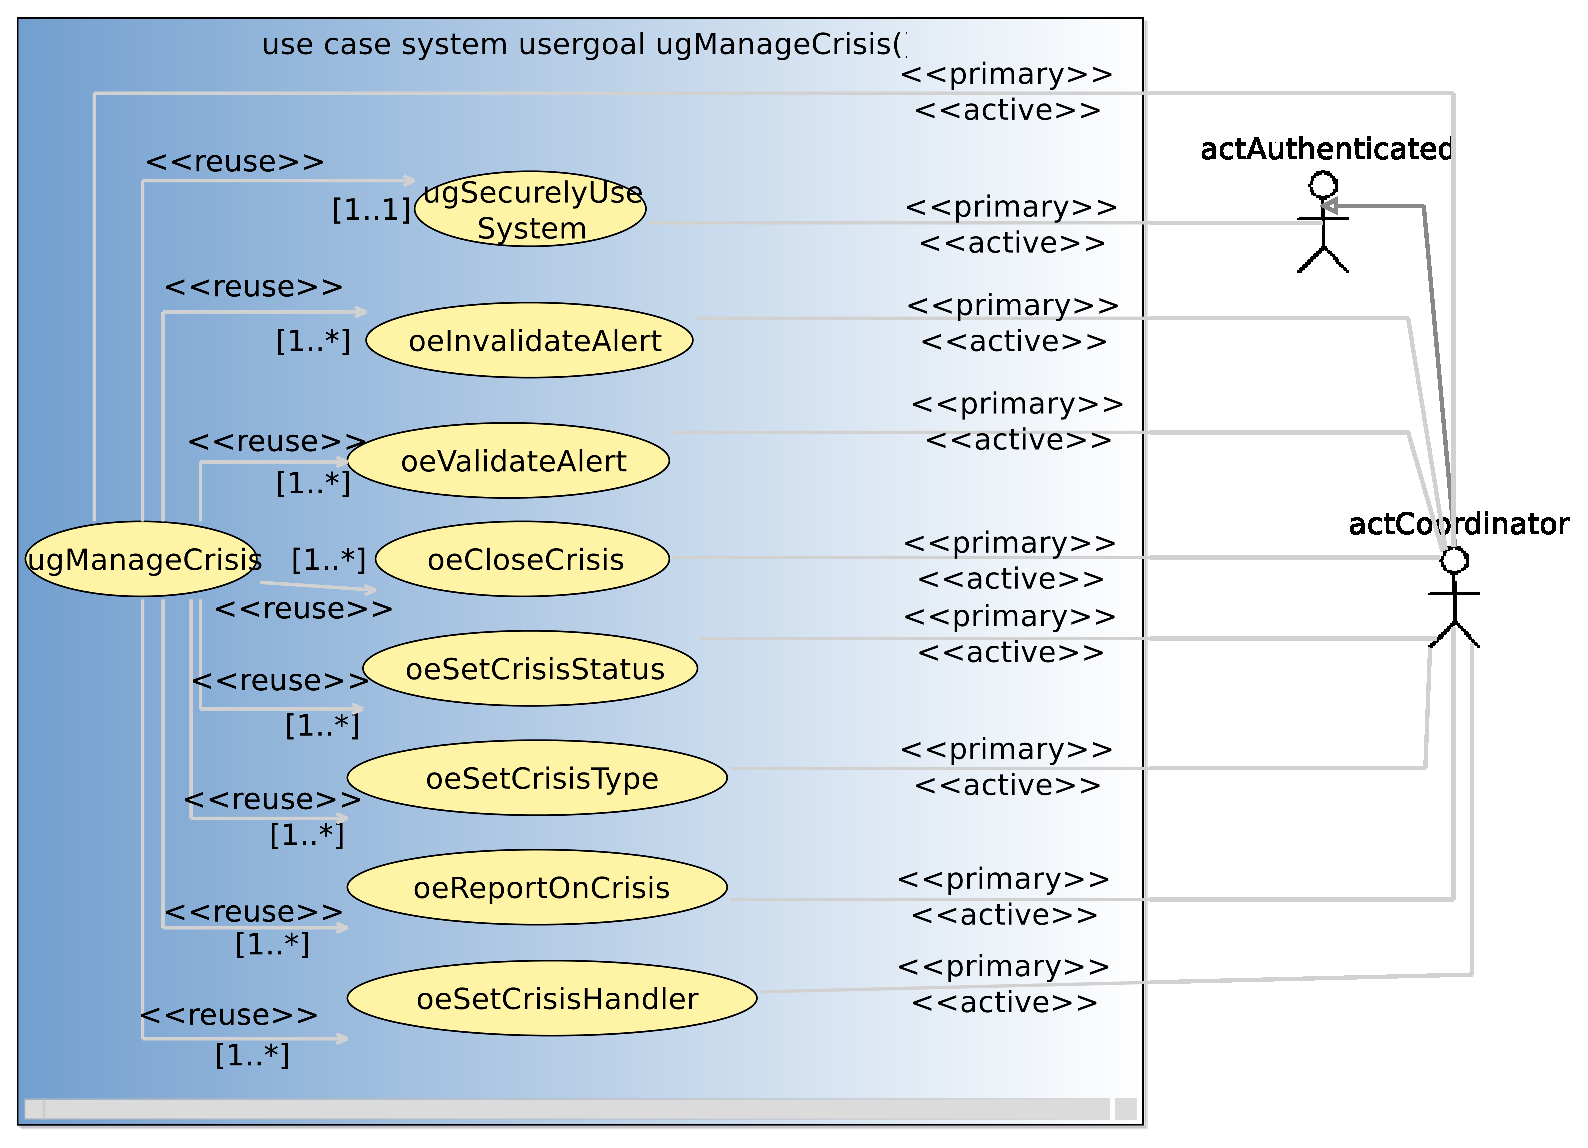
\includegraphics[
angle=0
]{./images-report-gen/usecase-model/usergoal/uc-ugManageCrisis.eps}
\end{center}
\caption[lu.uni.lassy.excalibur.MyCrash.G02 Use Case Diagram: uc-ugManageCrisis]{user goal Manage Crisis}
\label{fig:lu.uni.lassy.excalibur.MyCrash.G02-RE-UCD-uc-ugManageCrisis}
\end{figure}
\vspace{0.5cm}
